% vim: set tw=78 sts=2 sw=2 ts=8 aw et ai:
\documentclass[12pt]{article}

\usepackage[paper=a4paper, top=2cm, bottom=3cm, left=2.5cm, right=2.5cm]{geometry}

\usepackage{ucs}
\usepackage[utf8x]{inputenc}
\usepackage[english]{babel}
%\usepackage{hyperref}	  % use \url{http://$URL} or \href{http://$URL}{Name}
\usepackage{underscore}	  % underscores need not be escaped
\usepackage{subfigure}
\usepackage{verbatim}
\usepackage{float}
\usepackage{booktabs}     % professional tables
\usepackage{parskip}
\usepackage{wrapfig}

% Support for including graphics
\usepackage{graphicx}
\DeclareGraphicsExtensions{.pdf,.png,.jpg}

\title{Grand Report Title}

\author{Nicolae-Alexandru Ivan\\
Faculty of Automatic Control and Computers\\
University POLITEHNICA of Bucharest\\
Splaiul Independenței 313, Bucharest, Romania, 060042 \\
\emph{nicolae.ivan@stud.acs.upb.ro}}

\date{\today}

\begin{document}

\maketitle

\begin{abstract}
% vim: set tw=78 sts=2 sw=2 ts=8 aw et ai:
Insert abstract here.

\end{abstract}

\section{Introduction}
\label{sec:introduction}
% vim: set tw=78 sts=2 sw=2 ts=8 aw et ai:

The concept of virtualization first emerged in the 1960, when IBM developed the first operating systems which could run another operating system as a process\cite{IBM}. Since then, the subject has seen considerable progress. Most importantly, it has driven the development of future hardware platforms, with features dedicated to virtualization being present in many modern processors.

The evolution of embedded hardware have made this type of hardware suitable for many functions which were only performed in the past by desktop or server systems. These functions vary greatly, but are generally centred around server-like behaviour.

However, the advances made in hardware are not enough to qualify embedded devices as a viable alternative for traditional server hardware. Virtualization is necessary to enable separation between multiple execution environments. The main reasons for this are distributing functionality across various components, providing security through isolation and having the possibility of running software released under different licenses on the same machine. Moreover, it provides a level of hardware abstraction, resulting in less effort to make software portable between platforms.

ARM processors are a prime example of the evolution of embedded systems. The v7 family of CPUs possesses specialized extensions that facilitate virtualization.


\section{Virtualization}
\label{sec:virtualization}
% vim: set tw=78 sts=2 sw=2 ts=8 aw et ai:

Virtualization is a concept in which one or more execution environments are simulated through various techniques. These may include hardware and software partitioning, time-sharing, machine emulation and others.\cite{intr-virtualization}

It implies having a machine on which the virtualization takes place, called a \textbf{host machine}, and a firmware or software, called a \textbf{hypervisor} or virtual machine manager, that creates the virtualized or \textbf{guest machine}.

The guest executes its code, but instead of running directly on the underlying hardware, it has to pass through the hypervisor, which may decide to run the instructions on the hardware or modify them beforehand.

\subsection{Hypervisor types}
\label{subsec:hypertypes}

Depending on how they function, there are two types of hypervisors, as classified in \cite{formal-virt}:
\begin{itemize}
\item
\textbf{Type-1} also called \textbf{native} is a hypervisor that runs directly on top of hardware, while the guest machines are run as processes
\item
\textbf{Type-2} is a hypervisor which runs inside an operating system
\end{itemize}

\subsection{Types of virtualization}
\label{subsec:typesvirt}

In order to perform efficient virtualization, most instructions must be executed directly by the hardware. Interpreting the instructions would incur a performance drop\cite{virt-embedded}. 

However, not all instructions can be directly executed. There are two types of such instructions\cite{virt-embedded} :
\begin{itemize}
\item
\textbf{Control-sensitive instructions} which perform changes on hardware resources through various operations, e.g. I/O
\item
\textbf{Behaviour-sensitive instructions} which read the privilege level and might reveal to the guest that it is not running directly on hardware
\end{itemize}

Depending on how the framework handles sensitive instructions, there are two main types of virtualization\cite{vmware}:
\begin{enumerate}
\item
Full virtualization
\item
Paravirtualization
\end{enumerate}

\subsubsection{Full Virtualization}
\label{subsubsec:fullvirt}

This technique is composed of direct execution and binary translation.
As seen in Figure 1, user code is executed directly, while guest OS requests are translated into instructions that modify the virtual hardware.

In this case, the guest OS does not know it is being virtualized. Thus, no modifications to the operating system are necessary. The hypervisor may cache the translated instructions for future use.

\begin{figure}[h!]
\centering
  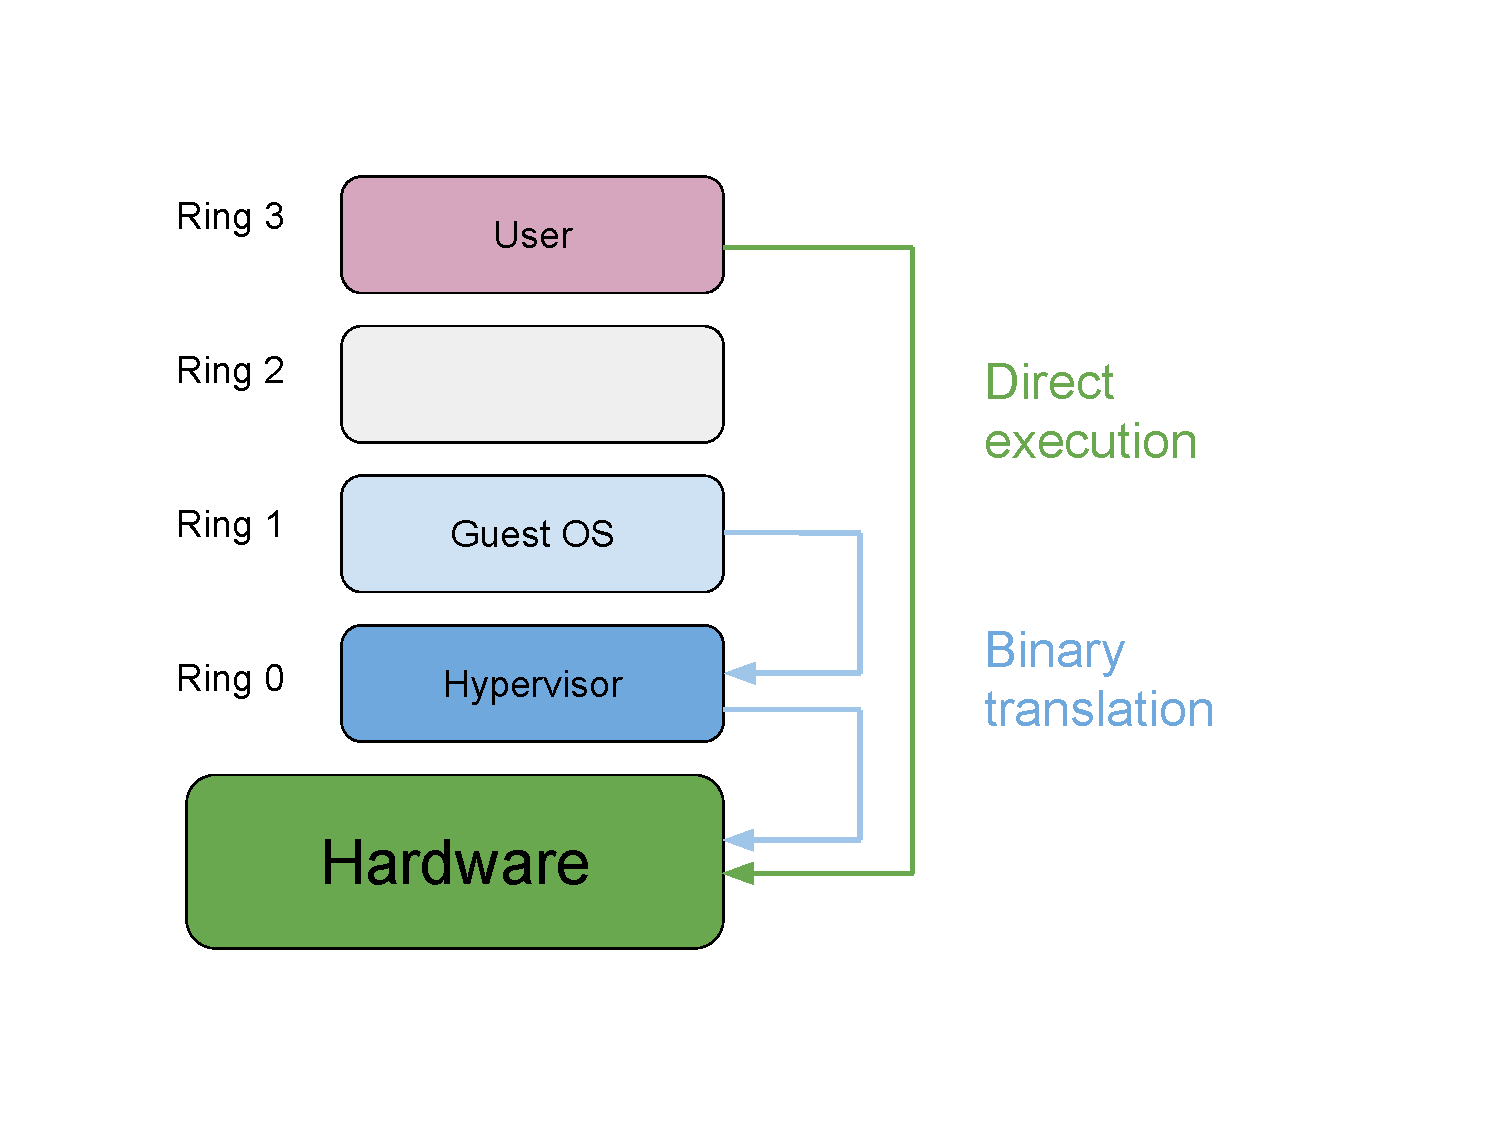
\includegraphics[width=.55\linewidth]{img/fullvirt.pdf}
  \caption{Full Virtualization}
\end{figure}

\subsubsection{Paravirtulization}
\label{subsubsec:paravirt}

Paravirtualization means the hypervisor provides interfaces for operations that are not virtualizable. Because of this, guest OS instructions are now replaced by hypercalls which interact with the virtualization layer.

This approach incurs less performance penalty, but it requires modifications to the operating system which is to be virtualized. In addition, it brings the advantage of being able to replace multiple consecutive sensitive instructions with a single hypercall, reducing the penalty induced by exceptions\cite{virt-embedded}.

\begin{figure}[h!]
\centering
  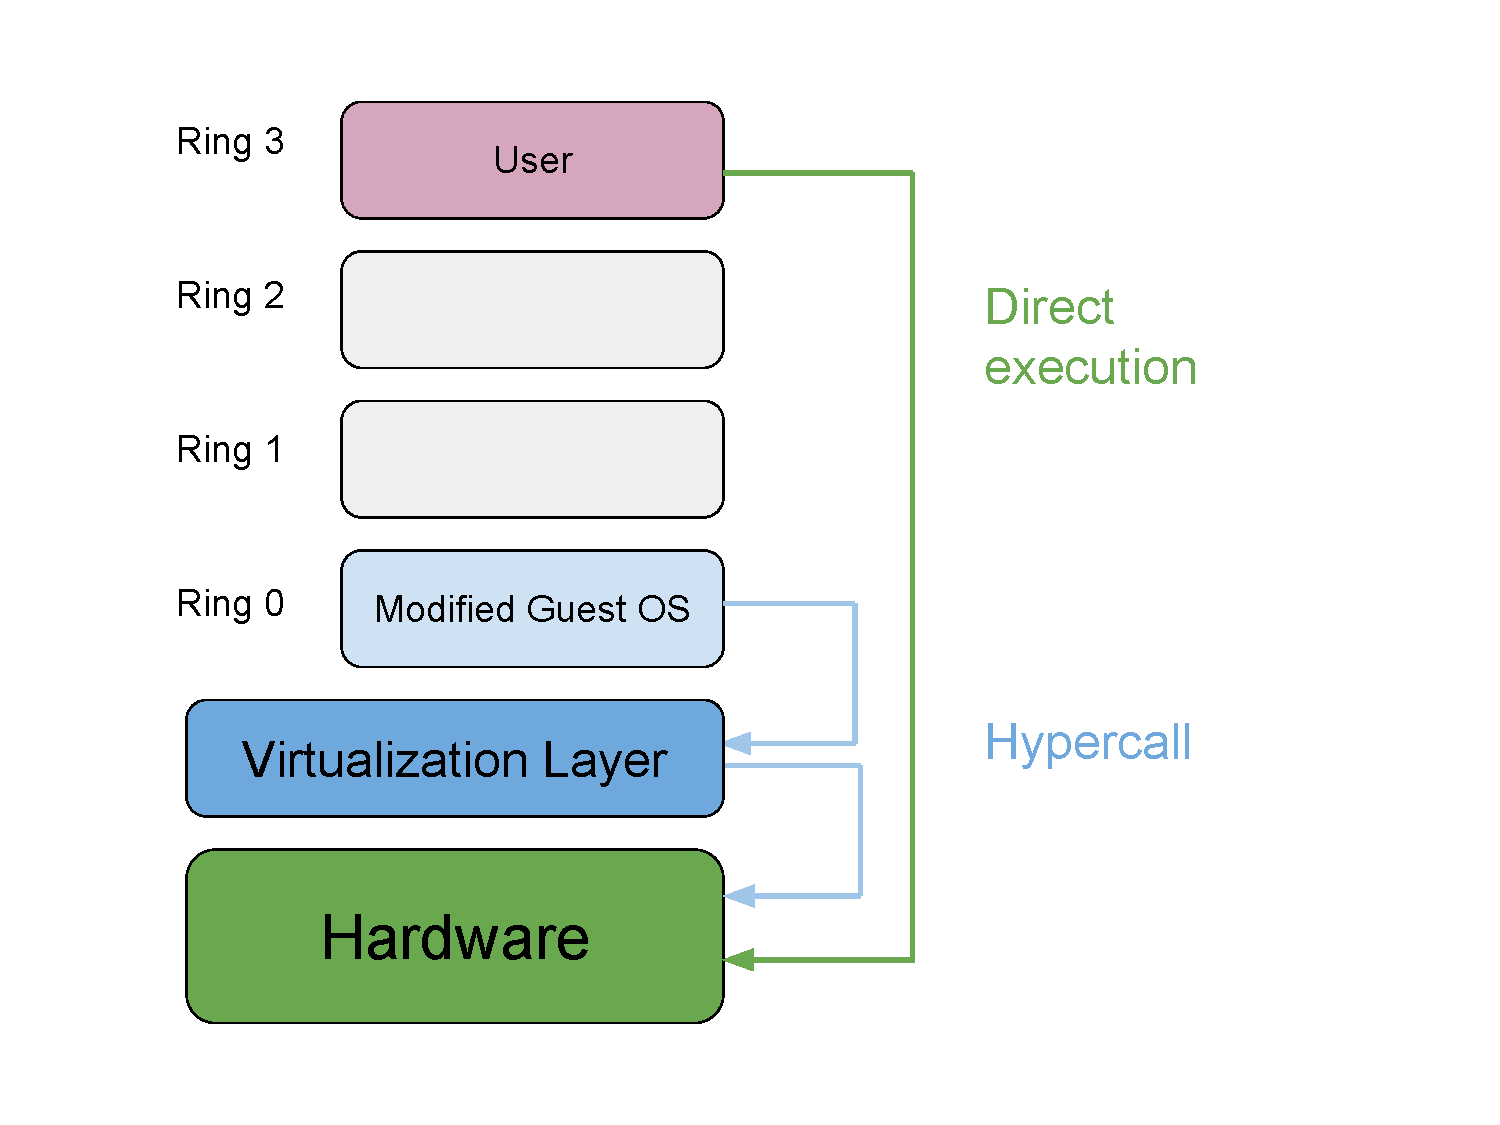
\includegraphics[width=.55\linewidth]{img/paravirt.pdf}
  \caption{Paravirtualization}
\end{figure}

\subsection{Hardware Assisted Virtualization}
\label{subsec:havirt}

In 2006, Intel release its VT-x and AMD presented AMD-V, both introducing the notion of hardware assisted virtualization. The feature consists of a new root level of privilege in which the virtual machine manager runs. Sensitive calls trap to this level without  translation or paravirtualization\cite{vmware}.

Memory is also virtualized in order to accommodate guest systems. This is done by an extra level of indirection in memory management. The memory management unit must map guest physical memory to host machine physical memory\cite{genode-arm}.

\subsection{Virtualization on ARM}
\label{subsec:armvirt}

ARM is a 32-bit RISC architecture. It features one user mode and 6 kernel modes. A secure mode is present, which can be used to protect access to hardware resources and a monitor mode also exists and is responsible for switching between the secure and normal modes\cite{hw-support-arm}.

ARM virtualization works similarly to Intel and AMD, in the sense that it also introduces a new privilege level, namely the \textbf{hyp} mode. In order to handle virtual memory usage while in this mode, an additional memory management unit was introduced. An additional extension, called Large Physical Address Extension, was also added, extending the addressable physical memory space to 40 bits\cite{genode-arm}.

\begin{figure}[h!]
\centering
  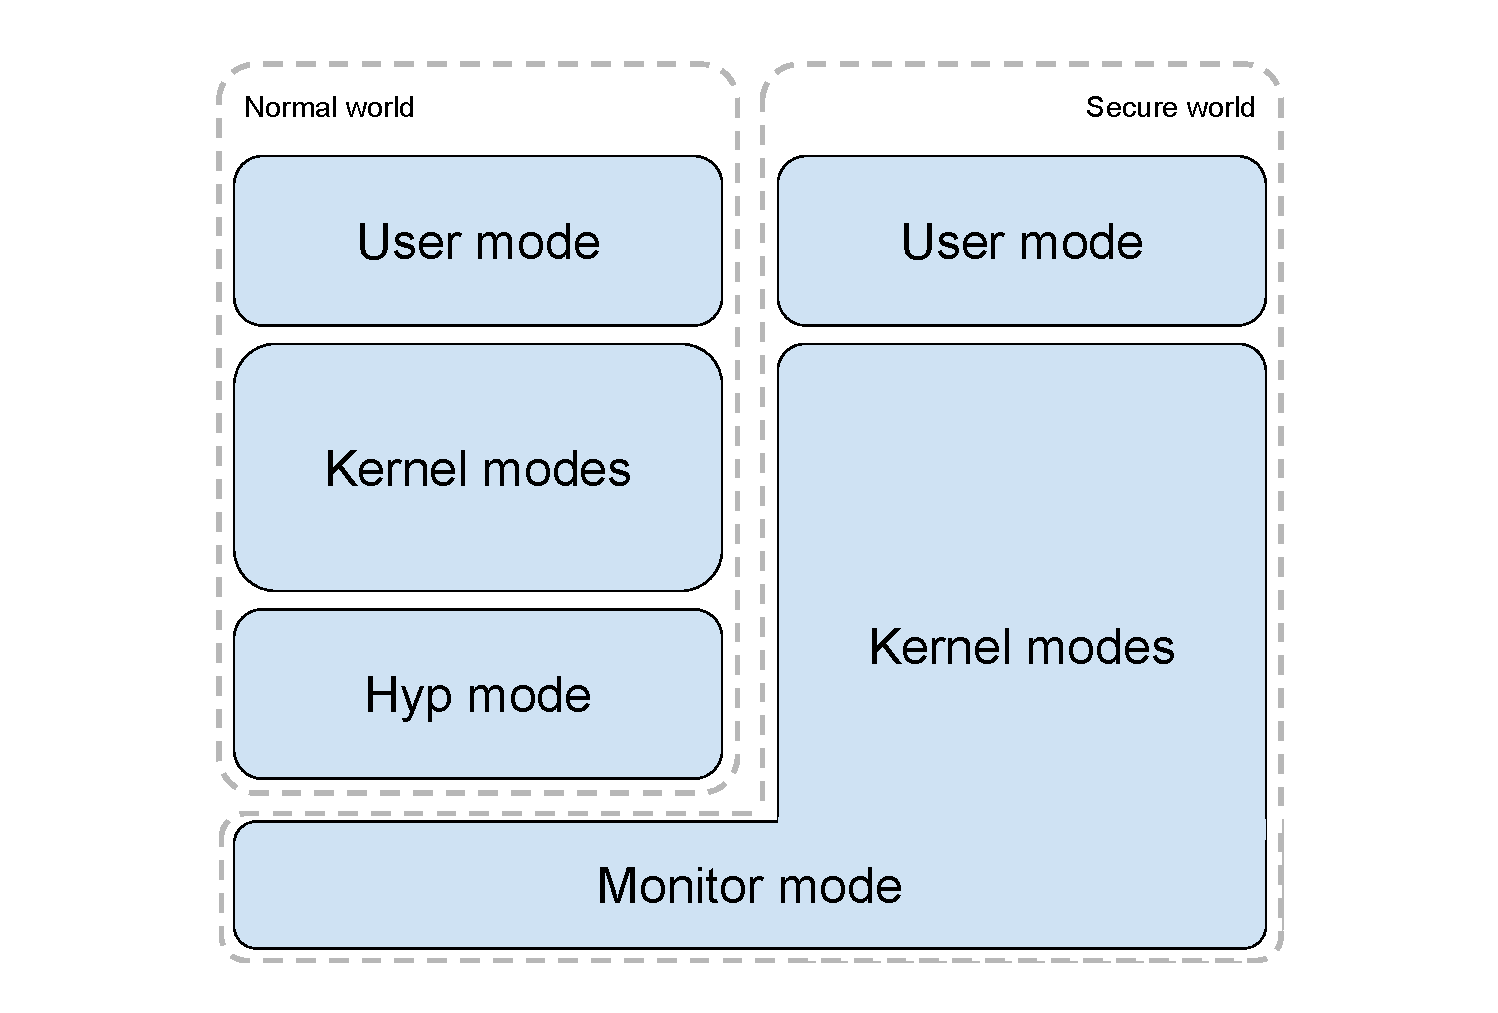
\includegraphics[width=.7\linewidth]{img/arm.pdf}
  \caption{ARM privilege levels}
\end{figure}

Another component introduced by ARM is called \textbf{virtual CPU} which allows virtual interrupts. Such interrupts can either be handled by the hypervisor, or linked directly to the physical interrupt\cite{hw-support-arm}.

\subsection{Advantages of Virtualization for Embedded Systems}
\label{subsec:advvirt}

Advances in performance of embedded systems have made them a viable platform for virtualization. The main reason why virtualization on embedded systems is necessary is to have multiple operating systems, each responsible for some subset of functions performed by the device.

Another important aspect of virtualization is the security benefits it brings. The isolation of one guest from another means that a vulnerability in one subsystem cannot lead to an exploit in another. This limits the possibilities a potential attacker has when trying to compromise a system\cite{virt-embedded}.

The above mentioned isolation also results in the possibility of using software distributed under different license agreements in different guests, while having efficient communication between these facilitated by the hypervisor.

\subsection{Limitations of Virtualization for Embedded Systems}
\label{subsec:limitvirt}

While performance of embedded systems has increased considerably, complexity of software systems has increased as well. The fact that each guest runs a separate operating system renders the virtual machines quite expensive from a resource perspective.

Another issue with performance is brought on by the scheduling mechanism. Due to the encapsulation of virtualized systems, the hypervisor can only associate a priority for each guest system. The result is that a higher priority machine will be preferred while scheduling, regardless of the priority of the task running inside the guest\cite{virt-embedded}.

Although virtualization does bring benefits in terms of security, it has some drawbacks. The increased amount of code on which a guest operating system relies on in order to function equates to increased amount of potential vulnerabilities.


\section{FreeBSD and bhyve}
\label{sec:bhyve}
% vim: set tw=78 sts=2 sw=2 ts=8 aw et ai:

\texttt{BSD} stands for "Berkeley Software Distribution". It is derived from AT\&T's Research UNIX operating system. In 1990, the BSD code was released without the proprietary AT\&T code.
Since the proprietary code contained a good portion of the kernel, it was not until 1992 that a complete operating system based on the BSD code was released - 386BSD. In 1993, the FreeBSD operating system split from the 386BSD project\cite{bsd}. 

\subsection{FreeBSD vs Linux}
\label{subsec:bsdlinux}

While FreeBSD originated from the UNIX systems, Linux was built to be a similar alternative for these. Therefore, they share many mechanisms, tools and applications.

The most significat difference between the two consists in the licensing. Linux is licensed under GNU General Public License(GPL)\cite{gnu}. This allows freedom to modify and redistribute the source code as long as it is also licensed under the GPL. FreeBSD is licensed under the BSD license, which is more permissive. It does not require derived work to maintain the license, but only to include a copy of the BSD license and original copyright\cite{bsd-license}.

Another difference consists of the available software. While most Linux distributions have little to no support for building software from source, FreeBSD provides an extensive collection of software source code which the user can customize and build. Conversely, while BSD maintainers are more conservative when modifying software packages, Linux distribution maintainers make modifications in order to improve component interconnection and management\cite{comp-bsd-linux}.

\subsection{bhyve}
\label{subsec:bhyve}

\texttt{bhyve} is an abbreviation for BSD hypervisor. It is a type-2 hypervisor, similar to Linux KVM. As of FreeBSD 10.0, it is part of the base system. It support various guest systems, ranging from other BSD systems to Linux distributions\cite{intr-bhyve}.

Being a legacy-free hypervisor, it is reliant on the virtualization features of CPUs. It requires both CPU and memory virtualization technologies.

bhyve has several components\cite{intr-bhyve}\cite{extending-bhyve}:
\begin{itemize}
\item
\textbf{vmm.ko} - kernel module, manages VT-x state, context switching, guest physical memory and other aspects
\item
\textbf{libvmmapi} - userland API
\item
\textbf{bhyveload} - userspace bootloader, creates vm and does initial setup, loads guest operating system
\item
\textbf{bhyve} - userspace run loop, emulates stdin/stdout, tap devices, block devices
\item
\textbf{bhyvectl} - utility that can modify virtual machine state; can also delete VMs
\end{itemize}

\begin{figure}[ht]
\centering
  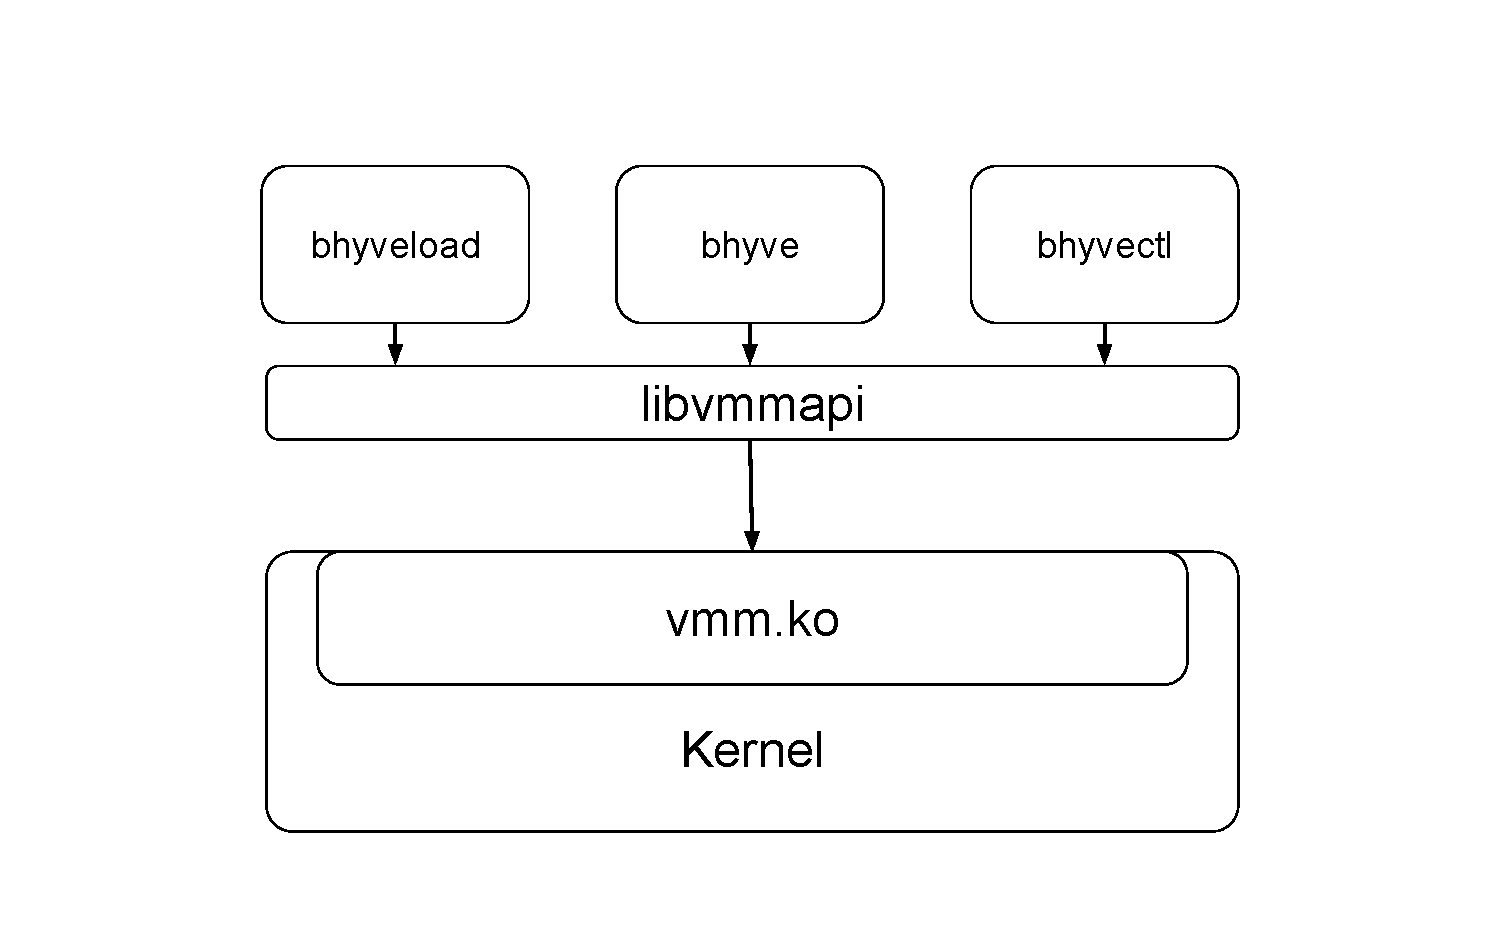
\includegraphics[width=.75\linewidth]{img/bhyve.pdf}
  \caption{bhyve overview}
\end{figure}


\section{Experimental Setup}
\label{sec:setup}
% vim: set tw=78 sts=2 sw=2 ts=8 aw et ai:

Before actually beginning to work on porting bhyve to ARMv7 a working baseline to compare future results to was needed. To this end, an Arndale Board was used. The board is based on a Samsung Exynos5250 processor, which is part of the ARMv7 family.
The two steps performed were:
\begin{itemize}
\item
Run FreeBSD on the Arndale board
\item
Run a KVM guest on a Linux host running on the Arndale board
\end{itemize}

\subsection{FreeBSD on Arndale}
\label{subsec:bsd-arndale}

This step was done in order to better understand the process of running FreeBSD on an ARM device. It was done by following the documentation from the FreeBSD wiki\cite{arndale}.
The setup has two important components to build: the FreeBSD system and the bootloader.

Building FreeBSD is a straightforward process. After obtaining the FreeBSD sources, one must simply build the kernel toolchain, provide the proper configuration, after which the kernel and the system can be built.

\begin{lstlisting}[frame=bottom, basicstyle=\footnotesize\ttfamily]
# make TARGET_ARCH=armv6 kernel-toolchain
# make TARGET_ARCH=armv6 KERNCONF=ARNDALE buildkernel
# make TARGET_ARCH=armv6 buildworld
# make TARGET_ARCH=armv6 DESTDIR=/mnt installworld distribution
\end{lstlisting}

The last command installs the filesystem in the /mnt directory.

Building the bootloader is also a simple process that consists of obtaining the source code, configuring and building the software.
The interesting part is preparing writing the bootloader to an SD card from which the board will boot. Three components are required:
\begin{itemize}
\item
\textbf{The stage one binary} - also called BL1, which is proprietary and does the first steps of the booting process
\item
\textbf{The secondary program loader} - or SPL, which is also board specific, although built by the bootloader; this component has the role of loading the actual bootloader
\item
\textbf{The u-boot binary} - this is the actual bootloader; it provides the needed functionality to load the kernel
\end{itemize}

With some minor issues, this step was performed successfully.

\subsection{KVM virtualization on Arndale}
\label{subsec:kvm-arndale}

The goal of this step was to establish a working baseline.
The approach used is described in the following guide\cite{kvm}.

There are many similarities to running FreeBSD on the Arndale board. Once more, the u-boot bootloader is used in order to load the kernel. However, in this case the kernel is a modified version of the 3.8 Linux kernel, with a patch set applied that enables KVM on ARM architecture. The filesystem for the host is built separately.

After booting the Linux host on the board, preparations for the running the guest systems must be made. The first part is to build \texttt{qemu}, which emulates devices and exposes KVM to userspace. Although a separate kernel has to be built for the guest system, the filesystem created for the host can be reused. Finally, the proper network configuration must be made in order to bridge the guest system network to the physical network.

This step proved to be more problematic than the previous. The main cause were modifications made in the repository for \texttt{qemu}, which resulted in attempting to compile multiple branches in order to obtain the proper binary. After several attempts, a decision was made to use the precompiled binary provided by the guide in order to save time. In the end, the process was successful.


\section{Scenarios and Results}
\label{sec:results}
% vim: set tw=78 sts=2 sw=2 ts=8 aw et ai:

The end justifies the means.


\section{Conclusion and Further Work}
\label{sec:conclusion}
% vim: set tw=78 sts=2 sw=2 ts=8 aw et ai:

And that was it.


\section*{Acknowledgment}
\label{sec:acknowledgment}

The authors would like to thank XYZ for their support and dedication.

\bibliographystyle{abbrv}
\bibliography{my-report}

\end{document}
